\PassOptionsToPackage{enable-debug,check-declarations}{expl3}
\RequirePackage{pdfmanagement-testphase}
\DeclareDocumentMetadata {  }
\ExplSyntaxOn
\pdfmanagement_add:nnn{Catalog}{Lang}{(enUS)}
\ExplSyntaxOff

% xmp metadata for pdf
% Originally used \usepackage[a-2a]{pdfx}
% \usepackage{hyperxmp} replaced it
% \RequirePackage{pdfmanagement-testphase} replaced it

\documentclass[11pt,
  english,
  a4paper,
]{article}
\usepackage{sa4ss}
\usepackage{amsmath,amssymb,array}
\usepackage{booktabs}

% From tagged-template.latex
\usepackage{lmodern}
\usepackage{ifxetex,ifluatex}
\ifnum 0\ifxetex 1\fi\ifluatex 1\fi=0 % if pdftex
  \usepackage[T1]{fontenc}
  \usepackage[utf8]{inputenc}
  \usepackage{textcomp} % provide euro and other symbols
\else % if luatex or xetex
  \usepackage{unicode-math}
  \defaultfontfeatures{Scale=MatchLowercase}
  \defaultfontfeatures[\rmfamily]{Ligatures=TeX,Scale=1}
\fi

% Use upquote if available, for straight quotes in verbatim environments
\IfFileExists{upquote.sty}{\usepackage{upquote}}{}
\IfFileExists{microtype.sty}{% use microtype if available
  \usepackage[]{microtype}
  \UseMicrotypeSet[protrusion]{basicmath} % disable protrusion for tt fonts
}{}
\makeatletter
\@ifundefined{KOMAClassName}{% if non-KOMA class
  \IfFileExists{parskip.sty}{%
    \usepackage{parskip}
  }{% else
    \setlength{\parindent}{0pt}
    \setlength{\parskip}{6pt plus 2pt minus 1pt}}
}{% if KOMA class
  \KOMAoptions{parskip=half}}
\makeatother
\usepackage{xcolor}
\IfFileExists{xurl.sty}{\usepackage{xurl}}{} % add URL line breaks if available
\hypersetup{
  pdftitle={DRAFT The status of Vermilion Rockfish (Sebastes miniatus) and Sunset Rockfish (Sebastes crocotulus) in U.S. waters off the coast of California south of Pt. Conception in 2021},
  pdflang={en},
  hidelinks,
  pdfcreator={LaTeX via pandoc}}
\urlstyle{same} % disable monospaced font for URLs
\usepackage{longtable}
% Correct order of tables after \paragraph or \subparagraph
\usepackage{etoolbox}
\makeatletter
\patchcmd\longtable{\par}{\if@noskipsec\mbox{}\fi\par}{}{}
\makeatother
% Allow footnotes in longtable head/foot
\IfFileExists{footnotehyper.sty}{\usepackage{footnotehyper}}{\usepackage{footnote}}
\makesavenoteenv{longtable}
\usepackage{graphicx}
\makeatletter
\def\maxwidth{\ifdim\Gin@nat@width>\linewidth\linewidth\else\Gin@nat@width\fi}
\def\maxheight{\ifdim\Gin@nat@height>\textheight\textheight\else\Gin@nat@height\fi}
\makeatother
% Scale images if necessary, so that they will not overflow the page
% margins by default, and it is still possible to overwrite the defaults
% using explicit options in \includegraphics[width, height, ...]{}
\setkeys{Gin}{width=\maxwidth,height=\maxheight,keepaspectratio}
% Set default figure placement to htbp
\makeatletter
\def\fps@figure{htbp}
\makeatother
\setlength{\emergencystretch}{3em} % prevent overfull lines
\providecommand{\tightlist}{%
  \setlength{\itemsep}{0pt}\setlength{\parskip}{0pt}}
\setcounter{secnumdepth}{5}
\usepackage{booktabs}
\usepackage{longtable}
\usepackage{array}
\usepackage{multirow}
\usepackage{wrapfig}
\usepackage{float}
\usepackage{colortbl}
\usepackage{pdflscape}
\usepackage{tabu}
\usepackage{threeparttable}
\usepackage[normalem]{ulem}
\usepackage{makecell}
\usepackage{placeins}
\ifxetex
  % Load polyglossia as late as possible: uses bidi with RTL langages (e.g. Hebrew, Arabic)
  \usepackage{polyglossia}
  \setmainlanguage[]{english}
\else
  \usepackage[shorthands=off,main=english]{babel}
\fi

%Define cslreferences environment, required by pandoc 2.8
%https://github.com/rstudio/rmarkdown/issues/1649
\newlength{\csllabelwidth}
\setlength{\csllabelwidth}{3em}
\newlength{\cslhangindent}
\setlength{\cslhangindent}{1.5em}
% for Pandoc 2.8 to 2.10.1
\newenvironment{cslreferences}%
  {}%
  {\par}
% For Pandoc 2.11+
\newenvironment{CSLReferences}[2] % #1 hanging-ident, #2 entry spacing
 {% don't indent paragraphs
  \setlength{\parindent}{0pt}
  % turn on hanging indent if param 1 is 1
  \ifodd #1 \everypar{\setlength{\hangindent}{\cslhangindent}}\ignorespaces\fi
  % set entry spacing
  \ifnum #2 > 0
  \setlength{\parskip}{#2\baselineskip}
  \fi
 }%
 {}
\usepackage{calc}  % for \widthof, \maxof in minipage
\newcommand{\CSLBlock}[1]{#1\hfill\break}
\newcommand{\CSLLeftMargin}[1]{\parbox[t]{\csllabelwidth}{#1}}
\newcommand{\CSLRightInline}[1]{\parbox[t]{\linewidth - \csllabelwidth}{#1}\break}
\newcommand{\CSLIndent}[1]{\hspace{\cslhangindent}#1}


\providecommand{\tightlist}{%
  \setlength{\itemsep}{0pt}\setlength{\parskip}{0pt}}

\usepackage{booktabs}
\usepackage{longtable}
\usepackage{array}
\usepackage{multirow}
\usepackage{wrapfig}
\usepackage{float}
\usepackage{colortbl}
\usepackage{pdflscape}
\usepackage{tabu}
\usepackage{threeparttable}
\usepackage[normalem]{ulem}
\usepackage{makecell}
\usepackage{placeins}
\date{}
\newcommand{\trTitle}{DRAFT The status of Vermilion Rockfish (\emph{Sebastes miniatus}) and Sunset Rockfish (\emph{Sebastes crocotulus}) in U.S. waters off the coast of California south of Pt. Conception in 2021}
\newcommand{\trYear}{2021}
\newcommand{\trMonth}{August}
\newcommand{\trAuthsLong}{truetruetruetruetrue}
\newcommand{\trAuthsBack}{Dick, E.J., M.H. Monk, T.L. Rogers, J.C. Field, E.M. Saas}
\newcommand{\trCitation}{
\begin{hangparas}{1em}{1}
\trAuthsBack{}. \trYear{}. \trTitle{}. Pacific Fisheries Management Council, Portland, Oregon. \pageref{LastPage}{}\,p.
\end{hangparas}}

\AtBeginDocument{\tagstructbegin{tag=Document}}
\AtEndDocument{\tagstructend}
\pretocmd{\maketitle}{\tagstructbegin{tag=H1}\tagmcbegin{tag=H1}}{}{}
\apptocmd{\maketitle}{\tagmcend\tagstructend}{}{}

\begin{document}

%%%%% Frontmatter %%%%%

% Footnote symbols in front matter
\renewcommand*{\thefootnote}{\fnsymbol{footnote}}

\small
\thispagestyle{empty}
\pagenumbering{roman}
\noindent
\begin{center}
\title{DRAFT The status of Vermilion Rockfish (\emph{Sebastes miniatus}) and Sunset Rockfish (\emph{Sebastes crocotulus}) in U.S. waters off the coast of California south of Pt. Conception in 2021}
% \textnormal{\MakeTextUppercase{\trTitle{}}}
\vspace{1.5cm}
{\Large\textbf\newline{DRAFT The status of Vermilion Rockfish (\emph{Sebastes miniatus}) and Sunset Rockfish (\emph{Sebastes crocotulus}) in U.S. waters off the coast of California south of Pt. Conception in 2021}}
\vfill
by\\
E. J. Dick\textsuperscript{1}\\
Melissa H. Monk\textsuperscript{1}\\
Tanya L. Rogers\textsuperscript{1}\\
John C. Field\textsuperscript{1}\\
Emma M. Saas\textsuperscript{2}\vfill
\textsuperscript{1}Southwest Fisheries Science Center, U.S. Department of Commerce, National Oceanic and Atmospheric Administration, National Marine Fisheries Service, 110 McAllister Way, Santa Cruz, California 95060\\
\textsuperscript{2}Fisheries Collaborative Program, Insitute of Marine Sciences, University of California, Santa Cruz, 110 McAllister Way, Santa Cruz, California 95060\vfill
\trMonth{} \trYear{}
\end{center}
\clearpage

% Fourth page: Colophon
\thispagestyle{empty}
\vspace*{\fill}
\begin{center}
\copyright{} Pacific Fisheries Management Council, \trYear{}\\
\end{center}
\par
\bigskip
\noindent
Correct citation for this publication:
\bigskip
\par
\trCitation{}
\clearpage

% Add TOC to pdf bookmarks (clickable pdf)
\pdfbookmark[1]{\contentsname}{toc}

% Table of contents page, lists of figures and tables
\tableofcontents\clearpage
\label{TRlastRoman}
\clearpage

% Table of contents
\newpage
\thispagestyle{empty} % to remove page number

% Settings for the main document
\pagenumbering{arabic}  % Regular page numbers
\pagestyle{plain}  % No page number on first page of main document, use 'empty'
\renewcommand*{\thefootnote}{\arabic{footnote}}  % Back to numeric footnotes
\setcounter{footnote}{0}  % And start at 1
\renewcommand{\headrulewidth}{0.5pt}
\renewcommand{\footrulewidth}{0.5pt}
%\pagestyle{fancy}\fancyhead[c]{Draft: Do not cite or circulate}

\newcommand{\lt}{\ensuremath <}
\newcommand{\gt}{\ensuremath >}

\newcommand\CapeM{$40^\circ 10^\prime N$}
\newcommand\PtC{$34^\circ 27^\prime N$}
\newcommand\CAOR{$42^\circ 00^\prime N$}

\newpage

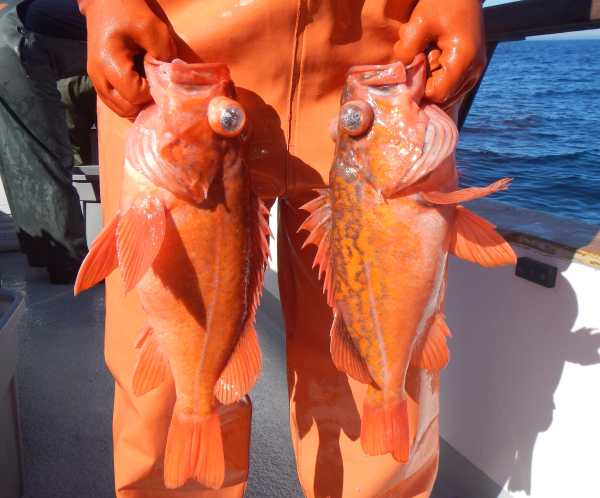
\includegraphics{cover_photo.png} Two fish of the vermilion/sunset cryptic species pair. Confirmation of species can only be determined via genetic analysis and species identification of these two fish caught in the Santa Barbara channel at approximately 250 ft depth is unknown. Photo courtesy of Sabrina Beyer.

\pagebreak
\pagenumbering{roman}
\setcounter{page}{1}

\renewcommand{\thetable}{\roman{table}}
\renewcommand{\thefigure}{\roman{figure}}

\setlength\parskip{0.5em plus 0.1em minus 0.2em}

\tagstructbegin{tag=H1}\tagmcbegin{tag=H1}

\hypertarget{executive-summary}{%
\section*{Executive Summary}\label{executive-summary}}
\addcontentsline{toc}{section}{Executive Summary}

\leavevmode\tagmcend\tagstructend

\tagstructbegin{tag=H2}\tagmcbegin{tag=H2}

\hypertarget{stock}{%
\subsection{Stock}\label{stock}}

\leavevmode\tagmcend\tagstructend

This assessment reports the status of the vermlion rockfish (\emph{Sebastes miniatus}) and sunset rockfish (\emph{Sebastes crocotulus}) complex (referred to as vermilion rockfish throughout), resource in U.S. waters off the coast of California south of Point Conception ($34^\circ 27^\prime N$) using data through 2020. Genetic evidence suggests a mixture of the two species with the majority of thee sunset rockfish population south of Point Conception. Alternative spatial structures for the vermilion rockfish assessment should be assessed if additional data on stock structure and the distribution of the two species become available.

\tagstructbegin{tag=H2}\tagmcbegin{tag=H2}

\hypertarget{catches}{%
\subsection*{Catches}\label{catches}}
\addcontentsline{toc}{subsection}{Catches}

\leavevmode\tagmcend\tagstructend

Over the past decade, vermilion rockfish off the coast of California have been primarily caught by the recreational fishery (Table \ref{tab:removalsES}). Annual total landings of catch and discards of vermilion rockfish have ranged between 106-260 mt, with landings (catch + discards) in 2020 totaling 110 mt. Vermilion and sunset rockfishes landings from all sectors have historically been recorded as ``vermilion rockfish'' and recreational sampling in California currently does not differentiate between the two species.

Recreational removals in California prior to 2004 were only estimated at large spatial scales (north and south of Point Conception) following the design of the Marine Recreational Fisheries Statistics Survey (MRFSS). Recent sampling (2004 -- present) by the California Recreational Fisheries Survey (CRFS) produces estimates of vermilion landings and discard at a finer spatial resolution. Total removals south of Point Conception increased steadily following World War II, peaking in the late 1970s and early 1980s with annual removals exceeding 398 mt per year (Figure \ref{fig:catch}). Recent years have seen a steady increase in landings, but total removals remain low relative to historical levels.

\FloatBarrier

\begin{figure}
\centering
\includegraphics[width=1\textwidth,height=1\textheight]{C:/Stock_Assessments/VRML_Assessment_2021/Model_files/SCA/Verm21SoCA_089_pre-STAR_base_with_SS_OPT/plots/catch2 landings stacked.png}
\caption{Catch histories by fleet used in the base model.\label{fig:catch}}
\end{figure}

\begin{table}[H]

\caption{\label{tab:removalsES}Recent landings by fleet, total landings summed across 
                fleets, and the total mortality including discards.}
\centering
\resizebox{\linewidth}{!}{
\begin{tabular}[t]{rrrrrrrrrr}
\toprule
Year & COM-HKL & COM-TWL & COM-NET & REC-PC & REC-PC-DIS & REC-PR & REC-PR-DIS & Total Landings & Total.Dead\\
\midrule
\cellcolor{gray!6}{2011} & \cellcolor{gray!6}{7.564} & \cellcolor{gray!6}{0.000} & \cellcolor{gray!6}{0.000} & \cellcolor{gray!6}{75.329} & \cellcolor{gray!6}{1.574} & \cellcolor{gray!6}{21.340} & \cellcolor{gray!6}{0.416} & \cellcolor{gray!6}{106.224} & \cellcolor{gray!6}{106.224}\\
2012 & 8.533 & 0.000 & 0.000 & 102.566 & 4.422 & 29.128 & 0.617 & 145.267 & 145.267\\
\cellcolor{gray!6}{2013} & \cellcolor{gray!6}{10.999} & \cellcolor{gray!6}{0.073} & \cellcolor{gray!6}{0.000} & \cellcolor{gray!6}{111.629} & \cellcolor{gray!6}{1.300} & \cellcolor{gray!6}{25.528} & \cellcolor{gray!6}{0.503} & \cellcolor{gray!6}{150.033} & \cellcolor{gray!6}{150.033}\\
2014 & 12.651 & 0.051 & 0.013 & 83.283 & 1.205 & 18.577 & 0.289 & 116.069 & 116.069\\
\cellcolor{gray!6}{2015} & \cellcolor{gray!6}{21.976} & \cellcolor{gray!6}{0.065} & \cellcolor{gray!6}{0.006} & \cellcolor{gray!6}{148.152} & \cellcolor{gray!6}{1.617} & \cellcolor{gray!6}{23.873} & \cellcolor{gray!6}{0.468} & \cellcolor{gray!6}{196.157} & \cellcolor{gray!6}{196.157}\\
\addlinespace
2016 & 16.099 & 0.171 & 0.056 & 129.384 & 0.813 & 25.279 & 0.328 & 172.129 & 172.129\\
\cellcolor{gray!6}{2017} & \cellcolor{gray!6}{33.287} & \cellcolor{gray!6}{0.115} & \cellcolor{gray!6}{0.022} & \cellcolor{gray!6}{89.956} & \cellcolor{gray!6}{1.189} & \cellcolor{gray!6}{25.282} & \cellcolor{gray!6}{0.250} & \cellcolor{gray!6}{150.102} & \cellcolor{gray!6}{150.102}\\
2018 & 40.246 & 0.034 & 0.039 & 82.319 & 1.909 & 17.211 & 0.355 & 142.112 & 142.112\\
\cellcolor{gray!6}{2019} & \cellcolor{gray!6}{47.217} & \cellcolor{gray!6}{0.291} & \cellcolor{gray!6}{0.045} & \cellcolor{gray!6}{172.463} & \cellcolor{gray!6}{5.296} & \cellcolor{gray!6}{33.640} & \cellcolor{gray!6}{1.020} & \cellcolor{gray!6}{259.971} & \cellcolor{gray!6}{259.971}\\
2020 & 48.764 & 0.075 & 0.096 & 38.880 & 1.576 & 19.828 & 0.461 & 109.680 & 109.680\\
\bottomrule
\end{tabular}}
\end{table}

\FloatBarrier

\tagstructbegin{tag=H2}\tagmcbegin{tag=H2}

\hypertarget{data-and-assessment}{%
\subsection*{Data and Assessment}\label{data-and-assessment}}
\addcontentsline{toc}{subsection}{Data and Assessment}

\leavevmode\tagmcend\tagstructend

This is the first full stock assessment for vermilion and sunset rockfishes. A full assessment was attempted in 2005, but not accepted for management and a data moderate assessment in 2013 was not reviewed. The 2021 assessment uses Stock Synthesis 3 (version V3.30.17.0). The assessment is a two sex model, with the population spanning from Point Conception to the California/Oregon border. The assessment model operates on an annual time step covering the period 1875 to 2020 (not including forecast years) and assumed an unfished population prior to 1875. Population dynamics are modeled for ages 0 through 70, with age-70 being the accumulator age.

The model is conditioned on catch from two sectors (commercial and recreational) divided among seven fleets, and is informed by five abundance indices (one fishery-independent survey, two CPUE indices from shore-based sampling programs, and two CPUE indices from onboard observer programs). Discards for the commercial fleet are not included in the model. Commercial discards of vermilion are a small fraction of the total mortality and data on commercial discard length composition is limited. The recreational fishery is split into four fleets, one discard and one retained fish fleet each for the private/rental and the party/charter boat modes.

The assessment estimates parameters for natural mortality of females and males, steepness of the Beverton-Holt stock-recruitment relationship, and sex-specific growth parameters. Year class strength is estimated as deviations from the expected stock-recruitment relationship beginning in 1965.

The assessment estimates parameters for natural mortality of females and males and sex-specific growth parameters. Year class strength is estimated as deviations from the expected stock-recruitment relationship beginning in 1965. Steepness of the Beverton-Holt stock-recruitment relationship is fixed at the mean of the prior, 0.72. A number of sources of uncertainty are addressed in this assessment. This assessment includes length data, estimated growth, an updated length-weight curve, an updated maturity curve, a number of new indices, and new conditional age-at-length data.

\FloatBarrier

\tagstructbegin{tag=H2}\tagmcbegin{tag=H2}

\hypertarget{stock-biomass}{%
\subsection*{Stock Biomass}\label{stock-biomass}}
\addcontentsline{toc}{subsection}{Stock Biomass}

\leavevmode\tagmcend\tagstructend

Spawning output of vermilion rockfish was estimated to be 465 million eggs in 2021 or 48\% of unfished spawning output (``depletion,'' Table \ref{tab:ssbES}). Depletion is a ratio of the estimated spawning output in a particular year relative to estimated unfished, equilibrium spawning output.

In southern California, spawning output declined rapidly in the 1970s and early 1980s, falling below the minimum stock size threshold in the early 1980s, followed by a steady recovery since the late 2000s (Figures \ref{fig:ssbES} and \ref{fig:deplES}). The trend in spawning output in 2017 is approaching the management target (40\% of unfished spawning output), but the precision of that estimate is low relative to other management reference points (e.g.~the SPR50\% proxies for target spawning output and maximum yield).

\begin{figure}
\centering
\includegraphics[width=1\textwidth,height=1\textheight]{C:/Stock_Assessments/VRML_Assessment_2021/Model_files/SCA/Verm21SoCA_089_pre-STAR_base_with_SS_OPT//plots/ts9_Relative_spawning_output_intervals.png}
\caption{Estimated time series of relative spawning output depletion (spawning output relative to unfished spawning output) with approximate 95\% asymptotic confidence intervals (dashed lines).\label{fig:deplES}}
\end{figure}

\begin{figure}
\centering
\includegraphics[width=1\textwidth,height=1\textheight]{C:/Stock_Assessments/VRML_Assessment_2021/Model_files/SCA/Verm21SoCA_089_pre-STAR_base_with_SS_OPT//plots/ts7_Spawning_output_with_95_asymptotic_intervals_intervals.png}
\caption{Estimated time series of spawning output with approximate 95\% asymptotic confidence intervals (dashed lines).\label{fig:ssbES}}
\end{figure}

\begin{table}[H]

\caption{\label{tab:ssbES}Estimated recent trend in spawning output and the fraction unfished and the 95 percent intervals.}
\centering
\resizebox{\linewidth}{!}{
\begin{tabular}[t]{rrrrrrr}
\toprule
Year & Spawning Output & Lower Interval & Upper Interval & Fraction Unfished & Lower Interval & Upper Interval\\
\midrule
\cellcolor{gray!6}{2011} & \cellcolor{gray!6}{417.626} & \cellcolor{gray!6}{216.763} & \cellcolor{gray!6}{618.489} & \cellcolor{gray!6}{0.427} & \cellcolor{gray!6}{0.232} & \cellcolor{gray!6}{0.622}\\
2012 & 417.703 & 217.755 & 617.651 & 0.427 & 0.234 & 0.620\\
\cellcolor{gray!6}{2013} & \cellcolor{gray!6}{416.626} & \cellcolor{gray!6}{217.570} & \cellcolor{gray!6}{615.682} & \cellcolor{gray!6}{0.426} & \cellcolor{gray!6}{0.235} & \cellcolor{gray!6}{0.617}\\
2014 & 418.821 & 219.116 & 618.526 & 0.428 & 0.238 & 0.619\\
\cellcolor{gray!6}{2015} & \cellcolor{gray!6}{428.176} & \cellcolor{gray!6}{225.337} & \cellcolor{gray!6}{631.015} & \cellcolor{gray!6}{0.438} & \cellcolor{gray!6}{0.245} & \cellcolor{gray!6}{0.631}\\
\addlinespace
2016 & 436.847 & 228.489 & 645.205 & 0.447 & 0.250 & 0.644\\
\cellcolor{gray!6}{2017} & \cellcolor{gray!6}{448.412} & \cellcolor{gray!6}{232.930} & \cellcolor{gray!6}{663.894} & \cellcolor{gray!6}{0.459} & \cellcolor{gray!6}{0.255} & \cellcolor{gray!6}{0.662}\\
2018 & 458.305 & 235.071 & 681.539 & 0.469 & 0.259 & 0.678\\
\cellcolor{gray!6}{2019} & \cellcolor{gray!6}{466.811} & \cellcolor{gray!6}{236.253} & \cellcolor{gray!6}{697.369} & \cellcolor{gray!6}{0.477} & \cellcolor{gray!6}{0.261} & \cellcolor{gray!6}{0.693}\\
2020 & 464.518 & 227.774 & 701.262 & 0.475 & 0.254 & 0.696\\
\addlinespace
\cellcolor{gray!6}{2021} & \cellcolor{gray!6}{471.178} & \cellcolor{gray!6}{228.525} & \cellcolor{gray!6}{713.831} & \cellcolor{gray!6}{0.482} & \cellcolor{gray!6}{0.256} & \cellcolor{gray!6}{0.708}\\
\bottomrule
\end{tabular}}
\end{table}

\FloatBarrier

\tagstructbegin{tag=H2}\tagmcbegin{tag=H2}

\hypertarget{recruitment}{%
\subsection*{Recruitment}\label{recruitment}}
\addcontentsline{toc}{subsection}{Recruitment}

\leavevmode\tagmcend\tagstructend

ajor recruitments (strong year classes) in southern California were consistently estimated by the primary sources of age data (NWFSC hook-and-line and trawl surveys), with a strong 1999 year class estimated even when either data set is removed (see sensitivity section). Other years with relatively high estimates of recruitment were 1983-84, 1999, and 2016 these are consistent with estimates of strong year classes in other rockfish stock assessments.

\begin{figure}
\centering
\includegraphics[width=1\textwidth,height=1\textheight]{C:/Stock_Assessments/VRML_Assessment_2021/Model_files/SCA/Verm21SoCA_089_pre-STAR_base_with_SS_OPT//plots/ts11_Age-0_recruits_(1000s)_with_95_asymptotic_intervals.png}
\caption{Age-0 recruits (1,000s) with \textasciitilde95\% asymptotic intervals.\label{fig:recruitsES}}
\end{figure}

\begin{table}[H]

\caption{\label{tab:recrES}Estimated recent trend in recruitment and recruitment deviations and the 95 percent intervals.}
\centering
\resizebox{\linewidth}{!}{
\begin{tabular}[t]{rrrrrrr}
\toprule
Year & Recruitment & Lower Interval & Upper Interval & Recruitment Deviations & Lower Interval & Upper Interval\\
\midrule
\cellcolor{gray!6}{2011} & \cellcolor{gray!6}{845.517} & \cellcolor{gray!6}{516.629} & \cellcolor{gray!6}{1383.777} & \cellcolor{gray!6}{0.248} & \cellcolor{gray!6}{-0.082} & \cellcolor{gray!6}{0.577}\\
2012 & 1025.460 & 643.904 & 1633.113 & 0.440 & 0.158 & 0.723\\
\cellcolor{gray!6}{2013} & \cellcolor{gray!6}{892.128} & \cellcolor{gray!6}{550.373} & \cellcolor{gray!6}{1446.097} & \cellcolor{gray!6}{0.302} & \cellcolor{gray!6}{-0.001} & \cellcolor{gray!6}{0.604}\\
2014 & 470.136 & 262.625 & 841.609 & -0.340 & -0.775 & 0.095\\
\cellcolor{gray!6}{2015} & \cellcolor{gray!6}{683.215} & \cellcolor{gray!6}{395.852} & \cellcolor{gray!6}{1179.184} & \cellcolor{gray!6}{0.030} & \cellcolor{gray!6}{-0.347} & \cellcolor{gray!6}{0.407}\\
\addlinespace
2016 & 1628.800 & 982.484 & 2700.287 & 0.895 & 0.574 & 1.216\\
\cellcolor{gray!6}{2017} & \cellcolor{gray!6}{1008.840} & \cellcolor{gray!6}{504.296} & \cellcolor{gray!6}{2018.176} & \cellcolor{gray!6}{0.405} & \cellcolor{gray!6}{-0.187} & \cellcolor{gray!6}{0.997}\\
2018 & 688.065 & 271.308 & 1745.005 & -0.039 & -0.924 & 0.845\\
\cellcolor{gray!6}{2019} & \cellcolor{gray!6}{743.171} & \cellcolor{gray!6}{274.415} & \cellcolor{gray!6}{2012.658} & \cellcolor{gray!6}{0.011} & \cellcolor{gray!6}{-0.955} & \cellcolor{gray!6}{0.978}\\
2020 & 747.805 & 275.049 & 2033.134 & 0.018 & -0.953 & 0.989\\
\addlinespace
\cellcolor{gray!6}{2021} & \cellcolor{gray!6}{736.076} & \cellcolor{gray!6}{272.812} & \cellcolor{gray!6}{1986.015} & \cellcolor{gray!6}{0.000} & \cellcolor{gray!6}{-0.980} & \cellcolor{gray!6}{0.980}\\
\bottomrule
\end{tabular}}
\end{table}

\FloatBarrier

\tagstructbegin{tag=H2}\tagmcbegin{tag=H2}

\hypertarget{exploitation-status}{%
\subsection*{Exploitation Status}\label{exploitation-status}}
\addcontentsline{toc}{subsection}{Exploitation Status}

\leavevmode\tagmcend\tagstructend

\begin{table}[H]

\caption{\label{tab:exploitES}Estimated recent trend in the (1-SPR)/(1-SPR 50\%) where SPR is the spawning potential ratio the exploitation rate, and the  95 percent intervals.}
\centering
\resizebox{\linewidth}{!}{
\begin{tabular}[t]{rrrrrrr}
\toprule
Year & (1-SPR)/(1-SPR 50\%) & Lower Interval & Upper Interval & Exploitation Rate & Lower Interval & Upper Interval\\
\midrule
\cellcolor{gray!6}{2011} & \cellcolor{gray!6}{0.935} & \cellcolor{gray!6}{0.632} & \cellcolor{gray!6}{1.237} & \cellcolor{gray!6}{0.119} & \cellcolor{gray!6}{0.068} & \cellcolor{gray!6}{0.169}\\
2012 & 1.063 & 0.745 & 1.380 & 0.150 & 0.087 & 0.213\\
\cellcolor{gray!6}{2013} & \cellcolor{gray!6}{1.000} & \cellcolor{gray!6}{0.686} & \cellcolor{gray!6}{1.313} & \cellcolor{gray!6}{0.130} & \cellcolor{gray!6}{0.075} & \cellcolor{gray!6}{0.184}\\
2014 & 0.795 & 0.518 & 1.072 & 0.093 & 0.054 & 0.132\\
\cellcolor{gray!6}{2015} & \cellcolor{gray!6}{1.134} & \cellcolor{gray!6}{0.805} & \cellcolor{gray!6}{1.464} & \cellcolor{gray!6}{0.154} & \cellcolor{gray!6}{0.088} & \cellcolor{gray!6}{0.221}\\
\addlinespace
2016 & 1.061 & 0.730 & 1.393 & 0.140 & 0.078 & 0.201\\
\cellcolor{gray!6}{2017} & \cellcolor{gray!6}{0.992} & \cellcolor{gray!6}{0.660} & \cellcolor{gray!6}{1.323} & \cellcolor{gray!6}{0.124} & \cellcolor{gray!6}{0.068} & \cellcolor{gray!6}{0.180}\\
2018 & 0.954 & 0.626 & 1.283 & 0.116 & 0.063 & 0.169\\
\cellcolor{gray!6}{2019} & \cellcolor{gray!6}{1.371} & \cellcolor{gray!6}{1.018} & \cellcolor{gray!6}{1.724} & \cellcolor{gray!6}{0.224} & \cellcolor{gray!6}{0.119} & \cellcolor{gray!6}{0.328}\\
2020 & 0.746 & 0.449 & 1.043 & 0.080 & 0.042 & 0.118\\
\bottomrule
\end{tabular}}
\end{table}

\begin{figure}
\centering
\includegraphics[width=1\textwidth,height=1\textheight]{C:/Stock_Assessments/VRML_Assessment_2021/Model_files/SCA/Verm21SoCA_089_pre-STAR_base_with_SS_OPT//plots/SPR3_ratiointerval.png}
\caption{Timeseries of SPR ratio: (1-SPR)/(1-SPR\_50\%).\label{fig:1-sprES}}
\end{figure}

\begin{figure}
\centering
\includegraphics[width=1\textwidth,height=1\textheight]{C:/Stock_Assessments/VRML_Assessment_2021/Model_files/SCA/Verm21SoCA_089_pre-STAR_base_with_SS_OPT//plots/ts_summaryF.png}
\caption{Time-series of estimated summary harvest rate (total catch divided by age-0 and older biomass) for the base case models with approximate 95\% asymptotic confidence intervals (grey lines).\label{fig:FmortalityES}}
\end{figure}

\begin{figure}
\centering
\includegraphics[width=1\textwidth,height=1\textheight]{C:/Stock_Assessments/VRML_Assessment_2021/Model_files/SCA/Verm21SoCA_089_pre-STAR_base_with_SS_OPT//plots/SPR4_phase.png}
\caption{Phase plot of the relative biomass (also referred to as fraction unfished) versus the SPR ratio where each point represents the biomass ratio at the start of the year and the relative fishing intensity in that same year. Lines through the final point show the 95 percent intervals based on the asymptotic uncertainty for each dimension. The shaded ellipse is a 95 percent region which accounts for the estimated correlations between the biomass ratio and SPR ratio.\label{fig:phaseES}}
\end{figure}

\begin{figure}
\centering
\includegraphics[width=1\textwidth,height=1\textheight]{C:/Stock_Assessments/VRML_Assessment_2021/Model_files/SCA/Verm21SoCA_089_pre-STAR_base_with_SS_OPT//plots/yield2_yield_curve_with_refpoints.png}
\caption{Equilibrium yield curve for the base case model. Values are based on the 2020 fishery selectivity.\label{fig:yield2ES}}
\end{figure}

\FloatBarrier

\tagstructbegin{tag=H2}\tagmcbegin{tag=H2}

\hypertarget{ecosystem-considerations}{%
\subsection*{Ecosystem Considerations}\label{ecosystem-considerations}}
\addcontentsline{toc}{subsection}{Ecosystem Considerations}

\leavevmode\tagmcend\tagstructend

In this assessment, ecosystem considerations were not explicitly included in the analysis.\\
This is primarily due to a lack of relevant data and results of analyses (conducted elsewhere) that could contribute ecosystem-related quantitative information for the assessment.

Vermilion/sunset rockfish are described as feeding on a wide range of both pelagic and benthic prey items, including forage fish species such as anchovies and mesopelagic fishes, squid, krill and octopus, as well as sporadically abundant pelagic organisms such as pyrosomes, salps and pelagic red crabs {\tagstructbegin{tag=Reference}\tagmcbegin{tag=Reference}(Phillips 1964, Love et al. 2002)\leavevmode\tagmcend\tagstructend}.

As with most other rockfish and groundfish in the California Current, recruitment, or cohort (year-class) strength appears to be highly variable for the vermilion/sunset rockfish complex, with only a modest apparent relationship to estimated levels of spawning output.\\
Oceanographic and ecosystem factors are widely recognized to be key drivers of recruitment variability for most species of groundfish, as well as most elements of California Current food webs. Although it is feasible that ecosystem factors, the results of pre-recruit surveys for co-occurring species, or the results of other groundfish assessments might ultimately be used to forecast recruitment for more data-limited stocks such as vermilion/sunset, as suggested by {\tagstructbegin{tag=Reference}\tagmcbegin{tag=Reference}(Thorson and Ward 2014)\leavevmode\tagmcend\tagstructend}, such approaches would require more development and evaluation. Consequently, environmental factors are not explicitly considered in this assessment.

\FloatBarrier

\tagstructbegin{tag=H2}\tagmcbegin{tag=H2}

\hypertarget{reference-points}{%
\subsection*{Reference Points}\label{reference-points}}
\addcontentsline{toc}{subsection}{Reference Points}

\leavevmode\tagmcend\tagstructend

Reference point and management quantities for the vermilion rockfish base case model can be found in Table \ref{tab:referenceES}. In 2020, spawning output relative to unfished spawning output (``depletion'') is estimated at 48\%. This stock assessment estimates that vermilion rockfish in the south is above the biomass target ({\tagstructbegin{tag=Formula}\tagmcbegin{tag=Formula}\(SB_{40\%}\)\leavevmode\tagmcend\tagstructend}), and well above the minimum stock size threshold ({\tagstructbegin{tag=Formula}\tagmcbegin{tag=Formula}\(SB_{25\%}\)\leavevmode\tagmcend\tagstructend}). Unfished age four-plus biomass is estimated to be 6010.98 mt in the base case model. The target spawning output ({\tagstructbegin{tag=Formula}\tagmcbegin{tag=Formula}\(SB_{40\%}\)\leavevmode\tagmcend\tagstructend}) is 391.134 million eggs, which corresponds with an equilibrium yield of 155.763 mt. Equilibrium yield at the proxy {\tagstructbegin{tag=Formula}\tagmcbegin{tag=Formula}\(F_{MSY}\)\leavevmode\tagmcend\tagstructend} harvest rate corresponding to {\tagstructbegin{tag=Formula}\tagmcbegin{tag=Formula}\(SPR_{50\%}\)\leavevmode\tagmcend\tagstructend} is 148.285 mt (Table \ref{tab:referenceES} and Figure \ref{fig:yield2ES}).

\begin{table}[H]

\caption{\label{tab:referenceES}Summary of reference points and management quantities including estimates of the 95 percent intervals.}
\centering
\resizebox{\linewidth}{!}{
\begin{tabular}[t]{lrrr}
\toprule
 & Estimate & Lower Interval & Upper Interval\\
\midrule
\cellcolor{gray!6}{Unfished Spawning Output} & \cellcolor{gray!6}{977.834} & \cellcolor{gray!6}{777.543} & \cellcolor{gray!6}{1178.125}\\
Unfished Age 4+ Biomass (mt) & 6010.980 & 4804.771 & 7217.189\\
\cellcolor{gray!6}{Unfished Recruitment (R0)} & \cellcolor{gray!6}{809.343} & \cellcolor{gray!6}{474.411} & \cellcolor{gray!6}{1144.275}\\
Spawning Output (2021) & 471.178 & 228.525 & 713.831\\
\cellcolor{gray!6}{Fraction Unfished (2021)} & \cellcolor{gray!6}{0.482} & \cellcolor{gray!6}{0.256} & \cellcolor{gray!6}{0.708}\\
\addlinespace
Reference Points Based SB40\% &  &  & \\
\cellcolor{gray!6}{Proxy Spawning Output SB40\%} & \cellcolor{gray!6}{391.134} & \cellcolor{gray!6}{311.018} & \cellcolor{gray!6}{471.250}\\
SPR Resulting in SB40\% & 0.456 & 0.380 & 0.531\\
\cellcolor{gray!6}{Exploitation Rate Resulting in SB40\%} & \cellcolor{gray!6}{0.139} & \cellcolor{gray!6}{0.106} & \cellcolor{gray!6}{0.172}\\
Yield with SPR Based On SB40\% (mt) & 155.763 & 124.738 & 186.788\\
\addlinespace
\cellcolor{gray!6}{Reference Points Based on SPR Proxy for MSY} & \cellcolor{gray!6}{} & \cellcolor{gray!6}{} & \cellcolor{gray!6}{}\\
Proxy Spawning Output (SPR50) & 439.020 & 356.091 & 521.949\\
\cellcolor{gray!6}{SPR50} & \cellcolor{gray!6}{0.500} & \cellcolor{gray!6}{} & \cellcolor{gray!6}{}\\
Exploitation Rate Corresponding to SPR50 & 0.121 & 0.107 & 0.136\\
\cellcolor{gray!6}{Yield with SPR50 at SB SPR (mt)} & \cellcolor{gray!6}{148.285} & \cellcolor{gray!6}{120.937} & \cellcolor{gray!6}{175.633}\\
\addlinespace
Reference Points Based on Estimated MSY Values &  &  & \\
\cellcolor{gray!6}{Spawning Output at MSY (SB MSY)} & \cellcolor{gray!6}{268.898} & \cellcolor{gray!6}{136.620} & \cellcolor{gray!6}{401.176}\\
SPR MSY & 0.342 & 0.163 & 0.521\\
\cellcolor{gray!6}{Exploitation Rate Corresponding to SPR MSY} & \cellcolor{gray!6}{0.195} & \cellcolor{gray!6}{0.092} & \cellcolor{gray!6}{0.298}\\
MSY (mt) & 165.171 & 124.402 & 205.940\\
\bottomrule
\end{tabular}}
\end{table}

\FloatBarrier

\tagstructbegin{tag=H2}\tagmcbegin{tag=H2}

\hypertarget{management-performance}{%
\subsection*{Management Performance}\label{management-performance}}
\addcontentsline{toc}{subsection}{Management Performance}

\leavevmode\tagmcend\tagstructend

Vermilion rockfish are managed as part of the minor shelf rockfish complex in the Pacific Coast Groundfish Fishery Management Plan. The total mortality of the minor shelf rockfish has been above the ACL in all years (2011-2019). Total mortality estimates from the NWFSC are not yet available for 2019-2020. A summary of these values as well as other base case summary results can be found in Tables \ref{tab:managementES} and \ref{tab:summaryES}.

\begin{table}

\caption{\label{tab:managementES}Annual estimates of total mortality, overfishing limit (OFL), acceptable biological catch (ABC), annual catch limit (ACL) for vermilion. The ABC is equal to the ACL.  Data were obtained from the GEMM reports.}
\centering
\resizebox{\linewidth}{!}{
\begin{tabular}[t]{lrrrrrrrrrrrr}
\toprule
 & 2011 & 2012 & 2013 & 2014 & 2015 & 2016 & 2017 & 2018 & 2019 & 2020 & 2021 & 2022\\
\midrule
\addlinespace[0.3em]
\multicolumn{13}{l}{\textbf{North of 40°10' N}}\\
\hspace{1em}OFL & 11.127 & 11.127 & 9.717 & 9.717 & 9.717 & 9.717 & 9.720 & 9.720 & 9.720 & 9.720 & 9.700 & 9.700\\
\hspace{1em}ABC & 5.564 & 5.564 & 8.104 & 8.104 & 8.104 & 8.104 & 8.104 & 8.104 & 8.104 & 8.104 & 7.547 & 7.547\\
\hspace{1em}Total landings & 15.249 & 18.695 & 14.149 & 10.504 & 13.472 & 12.104 & 20.602 & 22.949 & 25.696 &  &  & \\
\hspace{1em}CA rec landings & 4.209 & 4.867 & 2.657 & 2.950 & 5.018 & 4.549 & 6.490 & 7.631 & 7.884 &  &  & \\
\hspace{1em}OR rec landings & 6.102 & 9.150 & 6.305 & 3.949 & 4.653 & 3.689 & 8.798 & 9.199 & 9.252 &  &  & \\
\hspace{1em}WA rec landings & 1.001 & 0.911 & 1.279 & 0.960 & 1.141 & 0.997 & 0.731 & 1.151 & 2.497 &  &  & \\
\hspace{1em}Commercial landings & 3.935 & 3.767 & 3.906 & 2.644 & 2.661 & 2.799 & 4.557 & 4.966 & 6.063 &  &  & \\
\hspace{1em}Research & 0.002 &  & 0.002 & 0.002 &  & 0.069 & 0.026 & 0.002 &  &  &  & \\
\addlinespace[0.3em]
\multicolumn{13}{l}{\textbf{South of 40°10' N}}\\
\hspace{1em}OFL & 308.359 & 308.359 & 269.276 & 269.276 & 269.276 & 269.276 & 269.280 & 269.280 & 269.280 & 269.280 & 269.280 & 269.280\\
\hspace{1em}ABC & 154.179 & 154.179 & 224.576 & 224.576 & 224.576 & 224.576 & 224.580 & 224.580 & 224.580 & 224.580 & 209.515 & 209.515\\
\hspace{1em}Total Landings & 210.310 & 235.216 & 237.074 & 197.043 & 334.984 & 292.375 & 341.207 & 344.454 & 484.967 &  &  & \\
\hspace{1em}CA rec landings & 191.437 & 216.480 & 208.198 & 167.572 & 291.779 & 260.162 & 287.493 & 278.158 & 413.946 &  &  & \\
\hspace{1em}Commercial landings & 16.928 & 16.642 & 26.601 & 26.607 & 39.669 & 29.148 & 48.195 & 59.644 & 67.189 &  &  & \\
\hspace{1em}Research & 1.944 & 2.094 & 2.275 & 2.863 & 3.536 & 3.065 & 5.519 & 6.652 & 3.832 &  &  & \\
\bottomrule
\end{tabular}}
\end{table}

\begin{table}[H]

\caption{\label{tab:summaryES}Summary of recent estimates and managment quantities.}
\centering
\resizebox{\linewidth}{!}{
\begin{tabular}[t]{lrrrrrrrrrrr}
\toprule
Quantity & 2011 & 2012 & 2013 & 2014 & 2015 & 2016 & 2017 & 2018 & 2019 & 2020 & 2021\\
\midrule
\cellcolor{gray!6}{OFL} & \cellcolor{gray!6}{11.127} & \cellcolor{gray!6}{11.127} & \cellcolor{gray!6}{9.717} & \cellcolor{gray!6}{9.717} & \cellcolor{gray!6}{9.717} & \cellcolor{gray!6}{9.717} & \cellcolor{gray!6}{9.720} & \cellcolor{gray!6}{9.720} & \cellcolor{gray!6}{9.720} & \cellcolor{gray!6}{9.720} & \cellcolor{gray!6}{9.700}\\
ABC & 5.564 & 5.564 & 8.104 & 8.104 & 8.104 & 8.104 & 8.104 & 8.104 & 8.104 & 8.104 & 7.547\\
\cellcolor{gray!6}{Total Catch} & \cellcolor{gray!6}{106.224} & \cellcolor{gray!6}{145.267} & \cellcolor{gray!6}{150.033} & \cellcolor{gray!6}{116.069} & \cellcolor{gray!6}{196.157} & \cellcolor{gray!6}{172.129} & \cellcolor{gray!6}{150.102} & \cellcolor{gray!6}{142.112} & \cellcolor{gray!6}{259.971} & \cellcolor{gray!6}{109.680} & \cellcolor{gray!6}{}\\
(1-SPR)/(1-SPR 50\textbackslash{}\%) & 106.224 & 145.267 & 150.033 & 116.069 & 196.157 & 172.129 & 150.102 & 142.112 & 259.971 & 109.680 & \\
\cellcolor{gray!6}{(1-SPR)/(1-SPR\_50\%)} & \cellcolor{gray!6}{0.935} & \cellcolor{gray!6}{1.063} & \cellcolor{gray!6}{1.000} & \cellcolor{gray!6}{0.795} & \cellcolor{gray!6}{1.134} & \cellcolor{gray!6}{1.061} & \cellcolor{gray!6}{0.992} & \cellcolor{gray!6}{0.954} & \cellcolor{gray!6}{1.371} & \cellcolor{gray!6}{0.746} & \cellcolor{gray!6}{}\\
\addlinespace
Fill in F method & 0.119 & 0.150 & 0.130 & 0.093 & 0.154 & 0.140 & 0.124 & 0.116 & 0.224 & 0.080 & \\
\cellcolor{gray!6}{Age 4+ Biomass (mt)} & \cellcolor{gray!6}{2728.890} & \cellcolor{gray!6}{2792.570} & \cellcolor{gray!6}{2917.820} & \cellcolor{gray!6}{3082.180} & \cellcolor{gray!6}{3189.400} & \cellcolor{gray!6}{3249.510} & \cellcolor{gray!6}{3289.000} & \cellcolor{gray!6}{3242.810} & \cellcolor{gray!6}{3233.160} & \cellcolor{gray!6}{3321.640} & \cellcolor{gray!6}{6006.080}\\
Spawning Output & 417.626 & 417.703 & 416.626 & 418.821 & 428.176 & 436.847 & 448.412 & 458.305 & 466.811 & 464.518 & 471.178\\
\cellcolor{gray!6}{Lower Interval} & \cellcolor{gray!6}{216.763} & \cellcolor{gray!6}{217.755} & \cellcolor{gray!6}{217.570} & \cellcolor{gray!6}{219.116} & \cellcolor{gray!6}{225.337} & \cellcolor{gray!6}{228.489} & \cellcolor{gray!6}{232.930} & \cellcolor{gray!6}{235.071} & \cellcolor{gray!6}{236.253} & \cellcolor{gray!6}{227.774} & \cellcolor{gray!6}{228.525}\\
Upper Interval & 618.489 & 617.651 & 615.682 & 618.526 & 631.015 & 645.205 & 663.894 & 681.539 & 697.369 & 701.262 & 713.831\\
\addlinespace
\cellcolor{gray!6}{Recruits} & \cellcolor{gray!6}{845.517} & \cellcolor{gray!6}{1025.460} & \cellcolor{gray!6}{892.128} & \cellcolor{gray!6}{470.136} & \cellcolor{gray!6}{683.215} & \cellcolor{gray!6}{1628.800} & \cellcolor{gray!6}{1008.840} & \cellcolor{gray!6}{688.065} & \cellcolor{gray!6}{743.171} & \cellcolor{gray!6}{747.805} & \cellcolor{gray!6}{736.076}\\
Lower Interval & 516.629 & 643.904 & 550.373 & 262.625 & 395.852 & 982.484 & 504.296 & 271.308 & 274.415 & 275.049 & 272.812\\
\cellcolor{gray!6}{Upper Interval} & \cellcolor{gray!6}{1383.777} & \cellcolor{gray!6}{1633.113} & \cellcolor{gray!6}{1446.097} & \cellcolor{gray!6}{841.609} & \cellcolor{gray!6}{1179.184} & \cellcolor{gray!6}{2700.287} & \cellcolor{gray!6}{2018.176} & \cellcolor{gray!6}{1745.005} & \cellcolor{gray!6}{2012.658} & \cellcolor{gray!6}{2033.134} & \cellcolor{gray!6}{1986.015}\\
Fraction Unfished & 0.427 & 0.427 & 0.426 & 0.428 & 0.438 & 0.447 & 0.459 & 0.469 & 0.477 & 0.475 & 0.482\\
\cellcolor{gray!6}{Lower Interval} & \cellcolor{gray!6}{0.232} & \cellcolor{gray!6}{0.234} & \cellcolor{gray!6}{0.235} & \cellcolor{gray!6}{0.238} & \cellcolor{gray!6}{0.245} & \cellcolor{gray!6}{0.250} & \cellcolor{gray!6}{0.255} & \cellcolor{gray!6}{0.259} & \cellcolor{gray!6}{0.261} & \cellcolor{gray!6}{0.254} & \cellcolor{gray!6}{0.256}\\
\addlinespace
Upper Interval & 0.622 & 0.620 & 0.617 & 0.619 & 0.631 & 0.644 & 0.662 & 0.678 & 0.693 & 0.696 & 0.708\\
\bottomrule
\end{tabular}}
\end{table}

\FloatBarrier

\tagstructbegin{tag=H2}\tagmcbegin{tag=H2}

\hypertarget{unresolved-problems-and-major-uncertainties}{%
\subsection*{Unresolved Problems and Major Uncertainties}\label{unresolved-problems-and-major-uncertainties}}
\addcontentsline{toc}{subsection}{Unresolved Problems and Major Uncertainties}

\leavevmode\tagmcend\tagstructend

The stratification of assessment areas along the coast was based on consideration of population structure identified in genetic analyses, differences in historical exploitation, disparate availability of data sources and state specific regulations to mitigate the catch of overfished species affecting catch of co-occurring stocks like vermilion rockfish. The Panel discussed the potential for alternative stratification such as north and south of Cape Mendocino depending on the results of future analysis of population structure under the Saltonstall/Kennedy grant discussed in the assessment south of Point Conception to better understand the distribution of sunset rockfish, potential for hybridization and resolve considerations surrounding population structure apparent in vermilion rockfish. A more regional approach might allow for greater efficiency gained by fewer assessment areas, while accounting for key differences.

Natural mortality remains the primary axis of uncertainty across assessment areas. Additional collection of otoliths from across the range of the stock and ageing existing structures from the hook and line survey may help reduce uncertainty in the future.

\FloatBarrier

\tagstructbegin{tag=H2}\tagmcbegin{tag=H2}

\hypertarget{decision-table-and-forecasts}{%
\subsection*{Decision Table and Forecasts}\label{decision-table-and-forecasts}}
\addcontentsline{toc}{subsection}{Decision Table and Forecasts}

\leavevmode\tagmcend\tagstructend

The forecasts of stock abundance and yield were developed using the post-STAR base model, with the forecasted projections presented in Table \ref{tab:projectionES}. The total catches in 2021 and 2022 are set to the projected catch from the California Department of Fish and Wildlife (CDFW) by sector.

Uncertainty in the forecasts is based upon the three states of nature agreed upon at the STAR panel, reflecting a bivariate sensitivity analysis between natural mortality and steepness. Both natural moratlity (assumed females equal to males) and steepness were estimated in the base model.

For reference, the base model predicted sigma is 0.258. The buffers were calculated assuming a category 2 stock, with sigma = 1.0 and a {\tagstructbegin{tag=Formula}\tagmcbegin{tag=Formula}\(p^*\)\leavevmode\tagmcend\tagstructend} = 0.45. Alternative catch streams (rows in the table) assume sigma = 1.0 and a {\tagstructbegin{tag=Formula}\tagmcbegin{tag=Formula}\(p^*\)\leavevmode\tagmcend\tagstructend} = 0.4, and removals of long-term equilibrium catch with and without a buffer assuming sigma = 1.0 and a {\tagstructbegin{tag=Formula}\tagmcbegin{tag=Formula}\(p^*\)\leavevmode\tagmcend\tagstructend} = 0.45. The buffer multiplier with {\tagstructbegin{tag=Formula}\tagmcbegin{tag=Formula}\(p^*\)\leavevmode\tagmcend\tagstructend} = 0.45 ranges from 0.874 in 2023 ramping to 0.803 in 2032. The low state of nature assumes {\tagstructbegin{tag=Formula}\tagmcbegin{tag=Formula}\(M\)\leavevmode\tagmcend\tagstructend} = .1125 and {\tagstructbegin{tag=Formula}\tagmcbegin{tag=Formula}\(h\)\leavevmode\tagmcend\tagstructend} = 0.675, and the high state of nature asumes {\tagstructbegin{tag=Formula}\tagmcbegin{tag=Formula}\(M\)\leavevmode\tagmcend\tagstructend} = 0.1475 and {\tagstructbegin{tag=Formula}\tagmcbegin{tag=Formula}\(h\)\leavevmode\tagmcend\tagstructend} = 0.875.

Current medium-term forecasts based on the alternative states of nature project that the stock will remain above the target threshold of 40\% in 2032 in the base model and also the state of nature assuming higher productivity (Table \ref{tab:DecisionES}). In all scenarios of the low state of nature,\\
the stock remains below the target threshold of 40\% until throughout the forecast. The base model with the base catches results in an increasing stock over the period from 2023-2032. In all scenarios the catch significantly decreases from 2022 to 2023 in a all catch scenarios; assumed catch in 2022 is 210 mt, and 2023 cathes from the base model range from 121-148 mt.

\begin{table}[H]

\caption{\label{tab:projectionES}Projections of potential OFLs (mt), ABCs (mt), estimated spawning output and fraction unfished.}
\centering
\resizebox{\linewidth}{!}{
\begin{tabular}[t]{rrrrrr}
\toprule
Year & Predicted OFL (mt) & ABC Catch (mt) & Age 4+ Biomass (mt) & Spawning Output & Fraction Unfished\\
\midrule
\cellcolor{gray!6}{2021} & \cellcolor{gray!6}{169.293} & \cellcolor{gray!6}{169.293} & \cellcolor{gray!6}{3450.76} & \cellcolor{gray!6}{471.178} & \cellcolor{gray!6}{0.481859}\\
2022 & 168.096 & 168.096 & 3457.17 & 474.244 & 0.484994\\
\cellcolor{gray!6}{2023} & \cellcolor{gray!6}{166.360} & \cellcolor{gray!6}{145.399} & \cellcolor{gray!6}{3461.48} & \cellcolor{gray!6}{479.835} & \cellcolor{gray!6}{0.490712}\\
2024 & 165.792 & 143.410 & 3477.53 & 488.193 & 0.499260\\
\cellcolor{gray!6}{2025} & \cellcolor{gray!6}{165.412} & \cellcolor{gray!6}{141.758} & \cellcolor{gray!6}{3485.04} & \cellcolor{gray!6}{495.306} & \cellcolor{gray!6}{0.506534}\\
\addlinespace
2026 & 165.119 & 140.186 & 3487.73 & 500.637 & 0.511986\\
\cellcolor{gray!6}{2027} & \cellcolor{gray!6}{164.882} & \cellcolor{gray!6}{138.666} & \cellcolor{gray!6}{3487.35} & \cellcolor{gray!6}{504.314} & \cellcolor{gray!6}{0.515746}\\
2028 & 164.704 & 137.198 & 3485.62 & 506.676 & 0.518161\\
\cellcolor{gray!6}{2029} & \cellcolor{gray!6}{164.590} & \cellcolor{gray!6}{135.951} & \cellcolor{gray!6}{3483.70} & \cellcolor{gray!6}{508.092} & \cellcolor{gray!6}{0.519610}\\
2030 & 164.536 & 134.590 & 3482.23 & 508.879 & 0.520414\\
\addlinespace
\cellcolor{gray!6}{2031} & \cellcolor{gray!6}{164.548} & \cellcolor{gray!6}{133.284} & \cellcolor{gray!6}{3481.83} & \cellcolor{gray!6}{509.328} & \cellcolor{gray!6}{0.520873}\\
2032 & 164.625 & 132.194 & 3482.77 & 509.642 & 0.521195\\
\bottomrule
\end{tabular}}
\end{table}

\FloatBarrier

\begin{table}

\caption{\label{tab:DecisionES}Decision table summarizing 12year projections (2021 to 2032) for vermilion based on three alternative states of nature spanning quantiles of spawning output in 2021.  Columns range over low, medium, and high state of nature, and rows range over different assumptions of total catch levels corresponding to the forecast catches from each state of nature.  Catches in 2021 and 2022 are fixed at catches provided by the CDFW.}
\centering
\resizebox{\linewidth}{!}{
\begin{tabular}[t]{>{\centering\arraybackslash}p{1in}|>{}c|>{}c|>{}c|>{\centering\arraybackslash}p{.8in}>{\centering\arraybackslash}p{.8in}|>{\centering\arraybackslash}p{.8in}>{\centering\arraybackslash}p{.8in}|>{\centering\arraybackslash}p{.8in}>{\centering\arraybackslash}p{.8in}}
\toprule
\multicolumn{4}{c}{ } & \multicolumn{2}{c}{Low Productivity} & \multicolumn{2}{c}{Base Model} & \multicolumn{2}{c}{High Productivity} \\
\cmidrule(l{3pt}r{3pt}){5-6} \cmidrule(l{3pt}r{3pt}){7-8} \cmidrule(l{3pt}r{3pt}){9-10}
\multicolumn{4}{c}{ } & \multicolumn{2}{c}{M = 0.1125} & \multicolumn{2}{c}{M = 0.1302} & \multicolumn{2}{c}{M = 0.1475} \\
\multicolumn{4}{c}{ } & \multicolumn{2}{c}{h = 0.675} & \multicolumn{2}{c}{h = 0.730} & \multicolumn{2}{c}{h = 0.875} \\
\multicolumn{4}{c}{ } & \multicolumn{2}{c}{NLL = 1015.23} & \multicolumn{2}{c}{NLL = 1013.02} & \multicolumn{2}{c}{NLL = 1014.72} \\
\cmidrule(l{3pt}r{3pt}){5-6} \cmidrule(l{3pt}r{3pt}){7-8} \cmidrule(l{3pt}r{3pt}){9-10}
  & Year & Buffer & Catch (mt) & Spawning Output & Fraction Unfished & Spawning Output & Fraction Unfished & Spawning Output & Fraction Unfished\\
\midrule
 & 2021 & 1.000 & 210 & 406 & 0.355 & 471 & 0.482 & 581 & 0.642\\
\cmidrule{1-10}
 & 2022 & 1.000 & 210 & 407 & 0.357 & 474 & 0.485 & 585 & 0.646\\

 & 2023 & 0.874 & 139 & 408 & 0.358 & 477 & 0.488 & 589 & 0.651\\

 & 2024 & 0.865 & 137 & 411 & 0.360 & 482 & 0.493 & 595 & 0.658\\

 & 2025 & 0.857 & 136 & 413 & 0.361 & 485 & 0.496 & 599 & 0.662\\

 & 2026 & 0.849 & 135 & 413 & 0.362 & 487 & 0.498 & 601 & 0.664\\

 & 2027 & 0.841 & 134 & 413 & 0.362 & 488 & 0.499 & 601 & 0.664\\

 & 2028 & 0.833 & 133 & 413 & 0.362 & 489 & 0.500 & 600 & 0.663\\

 & 2029 & 0.826 & 132 & 414 & 0.362 & 490 & 0.501 & 599 & 0.661\\

 & 2030 & 0.818 & 131 & 415 & 0.363 & 491 & 0.502 & 597 & 0.659\\

 & 2031 & 0.810 & 130 & 417 & 0.365 & 491 & 0.503 & 594 & 0.657\\

 & 2032 & 0.803 & 129 & 419 & 0.367 & 493 & 0.504 & 592 & 0.654\\

\multirow{-12}{1in}{\centering\arraybackslash P* = 0.45, sigma = 1} & 2021 & 1.000 & 210 & 406 & 0.355 & 471 & 0.482 & 581 & 0.642\\
\cmidrule{1-10}
 & 2022 & 1.000 & 210 & 407 & 0.357 & 474 & 0.485 & 585 & 0.646\\

 & 2023 & 0.762 & 121 & 408 & 0.358 & 477 & 0.488 & 589 & 0.651\\

 & 2024 & 0.747 & 119 & 413 & 0.362 & 484 & 0.495 & 598 & 0.660\\

 & 2025 & 0.733 & 118 & 418 & 0.366 & 490 & 0.501 & 604 & 0.667\\

 & 2026 & 0.719 & 116 & 421 & 0.368 & 495 & 0.506 & 608 & 0.672\\

 & 2027 & 0.706 & 115 & 424 & 0.371 & 499 & 0.510 & 611 & 0.675\\

 & 2028 & 0.693 & 114 & 427 & 0.374 & 503 & 0.514 & 613 & 0.677\\

 & 2029 & 0.680 & 112 & 432 & 0.378 & 506 & 0.518 & 614 & 0.678\\

 & 2030 & 0.667 & 111 & 437 & 0.382 & 510 & 0.522 & 615 & 0.679\\

 & 2031 & 0.654 & 109 & 442 & 0.387 & 515 & 0.526 & 616 & 0.680\\

 & 2032 & 0.642 & 108 & 448 & 0.392 & 519 & 0.531 & 617 & 0.681\\

\multirow{-12}{1in}{\centering\arraybackslash P* = 0.40, sigma = 1} & 2021 & 1.000 & 210 & 406 & 0.355 & 471 & 0.482 & 581 & 0.642\\
\cmidrule{1-10}
 & 2022 & 1.000 & 210 & 407 & 0.357 & 474 & 0.485 & 585 & 0.646\\

 & 2023 & 1.000 & 148 & 408 & 0.358 & 477 & 0.488 & 589 & 0.651\\

 & 2024 & 1.000 & 148 & 413 & 0.362 & 484 & 0.495 & 598 & 0.660\\

 & 2025 & 1.000 & 148 & 416 & 0.364 & 488 & 0.499 & 603 & 0.665\\

 & 2026 & 1.000 & 148 & 415 & 0.364 & 490 & 0.501 & 604 & 0.667\\

 & 2027 & 1.000 & 148 & 413 & 0.362 & 489 & 0.500 & 602 & 0.665\\

 & 2028 & 1.000 & 148 & 409 & 0.358 & 486 & 0.497 & 598 & 0.660\\

 & 2029 & 1.000 & 148 & 405 & 0.354 & 482 & 0.493 & 592 & 0.654\\

 & 2030 & 1.000 & 148 & 399 & 0.350 & 477 & 0.488 & 584 & 0.646\\

 & 2031 & 1.000 & 148 & 393 & 0.345 & 471 & 0.482 & 576 & 0.637\\

 & 2032 & 1.000 & 148 & 388 & 0.339 & 466 & 0.476 & 568 & 0.628\\

\multirow{-12}{1in}{\centering\arraybackslash Long-term Equil. Yield (MSY proxy, SPR50\%), no buffer} & 2021 & 1.000 & 210 & 406 & 0.355 & 471 & 0.482 & 581 & 0.642\\
\cmidrule{1-10}
 & 2022 & 1.000 & 210 & 407 & 0.357 & 474 & 0.485 & 585 & 0.646\\

 & 2023 & 0.874 & 130 & 408 & 0.358 & 477 & 0.488 & 589 & 0.651\\

 & 2024 & 0.865 & 128 & 415 & 0.364 & 486 & 0.497 & 599 & 0.662\\

 & 2025 & 0.857 & 127 & 420 & 0.368 & 493 & 0.504 & 607 & 0.670\\

 & 2026 & 0.849 & 126 & 423 & 0.370 & 497 & 0.508 & 611 & 0.675\\

 & 2027 & 0.841 & 125 & 424 & 0.372 & 500 & 0.511 & 612 & 0.676\\

 & 2028 & 0.833 & 124 & 425 & 0.372 & 501 & 0.512 & 611 & 0.675\\

 & 2029 & 0.826 & 123 & 425 & 0.372 & 501 & 0.512 & 609 & 0.673\\

 & 2030 & 0.818 & 122 & 424 & 0.371 & 500 & 0.511 & 606 & 0.669\\

 & 2031 & 0.810 & 121 & 424 & 0.371 & 499 & 0.510 & 602 & 0.665\\

\multirow{-11}{1in}{\centering\arraybackslash Long-term Equil. Yield (MSY proxy, SPR50\%), with buffer} & 2032 & 0.803 & 120 & 423 & 0.371 & 498 & 0.509 & 598 & 0.660\\
\bottomrule
\end{tabular}}
\end{table}

\newpage

\tagstructbegin{tag=H2}\tagmcbegin{tag=H2}

\hypertarget{research-and-data-needs}{%
\subsection*{Research and Data Needs}\label{research-and-data-needs}}
\addcontentsline{toc}{subsection}{Research and Data Needs}

\leavevmode\tagmcend\tagstructend

There are several areas for further research that were identified while conducting this assessment that could result in information useful to future vermilion and sunset rockfish assessments. The list below is believed to represent strategic pieces of information that would likely help to resolve key uncertainties associated with assessing either or both species. Many would provide the necessary information to evaluate basic life history parameters and spatiotemporal population and fleet dynamics.

\tagstructbegin{tag=L}

\begin{itemize}
\item
  Investigate the structure of complex and contribution of each species to the vermilion/sunset complex. Investigate possible spatial differences in biological parameters within a single species and also between the two species. Little biological data for south of Point Conception or north of Point Arena were available for this assessment and is needed to better under biological parameters.

  \tagstructbegin{tag=L}

  \begin{itemize}
  \item
    \tagstructbegin{tag=LI}\tagstructbegin{tag=LBody}\tagmcbegin{tag=P}

    \tagstructbegin{tag=LI}\tagstructbegin{tag=LBody}\tagmcbegin{tag=P}

    Conduct life history studies

    \tagmcend\tagstructend\tagstructend

    \tagmcend\tagstructend\tagstructend
  \item
    \tagstructbegin{tag=LI}\tagstructbegin{tag=LBody}\tagmcbegin{tag=P}

    \tagstructbegin{tag=LI}\tagstructbegin{tag=LBody}\tagmcbegin{tag=P}

    Conduct research to identify the proportion of each species in population and in catches

    \tagmcend\tagstructend\tagstructend

    \tagmcend\tagstructend\tagstructend
  \end{itemize}

  \tagstructend
\item
  Take a closer look at historical catch reconstructions and all other historical data sources.
\item
  Refine CCFRP survey index to look at alternative possible model structures, including a hierarchical structure and random effects. The CCFRP survey is the only fishery-independent survey available for nearshore rockfish sampling the nearshore rocky reef habitats. As of this assessment, only two years of coastwide data are available, and the index was limited to the site in central California that have been monitored since 2007.
\item
  Continue to investigate the most appropriate model structure for the NWFSC HL survey index. The NWFSC HL survey is the only long-term fishery-independent survey in rocky (untrawlable) habitat in the Southern California Bight. We also recommend evaluating how to structure the NWFSC Hook-and-Line survey index given its expansion into the CCA, also independent analysis of information content in NWFSC Hook-and-Line survey.Increased spatiotemporal sampling around Pt. Conception would aid in identifying stock boundaries.
\item
  Utilize existing ROV survey data sources

  \tagstructbegin{tag=L}

  \begin{itemize}
  \item
    \tagstructbegin{tag=LI}\tagstructbegin{tag=LBody}\tagmcbegin{tag=P}

    \tagstructbegin{tag=LI}\tagstructbegin{tag=LBody}\tagmcbegin{tag=P}

    SWFSC Submersible Survey of the Cowcod Conservation Areas {\tagstructbegin{tag=Reference}\tagmcbegin{tag=Reference}(Yoklavich et al. 2007)\leavevmode\tagmcend\tagstructend}.

    \tagmcend\tagstructend\tagstructend

    \tagmcend\tagstructend\tagstructend
  \item
    \tagstructbegin{tag=LI}\tagstructbegin{tag=LBody}\tagmcbegin{tag=P}

    \tagstructbegin{tag=LI}\tagstructbegin{tag=LBody}\tagmcbegin{tag=P}

    This was a line-transect survey designed to estimate cowcod abundance in 2002 conducted from a submersible inside the CCAs. Originally, only cowcod were enumerated from the video footage. Over the last few years, the SWFSC has re-analyzed the video footage to enumerate other rockfish species.

    \tagmcend\tagstructend\tagstructend

    \tagmcend\tagstructend\tagstructend
  \item
    \tagstructbegin{tag=LI}\tagstructbegin{tag=LBody}\tagmcbegin{tag=P}

    \tagstructbegin{tag=LI}\tagstructbegin{tag=LBody}\tagmcbegin{tag=P}

    The SWFSC Fishery Resource Division (FRD) conducted a survey of potential cowcod habitat between Point Conception and the U.S. -- Mexico border from October through December of 2012 {\tagstructbegin{tag=Reference}\tagmcbegin{tag=Reference}(Stierhoff and Cutter 2013)\leavevmode\tagmcend\tagstructend}.

    \tagmcend\tagstructend\tagstructend

    \tagmcend\tagstructend\tagstructend
  \item
    \tagstructbegin{tag=LI}\tagstructbegin{tag=LBody}\tagmcbegin{tag=P}

    \tagstructbegin{tag=LI}\tagstructbegin{tag=LBody}\tagmcbegin{tag=P}

    SWFSC staff are submitting proposals to conduct an additional submersible survey in the southern California Bight

    \tagmcend\tagstructend\tagstructend

    \tagmcend\tagstructend\tagstructend
  \item
    \tagstructbegin{tag=LI}\tagstructbegin{tag=LBody}\tagmcbegin{tag=P}

    \tagstructbegin{tag=LI}\tagstructbegin{tag=LBody}\tagmcbegin{tag=P}

    CDFW ROV survey data

    \tagmcend\tagstructend\tagstructend

    \tagmcend\tagstructend\tagstructend
  \end{itemize}

  \tagstructend
\item
  Collection of length and age data are recommended for both the commercial and recreational fisheries. Very little age data are available from either fishery for vermilion and sunset rockfishes.
\item
  Investigate possible environmental drivers/co-variates for biological parameters, particularly for recruitment.
\item
  Resolve differences between CalCOM and PacFIN expanded length composition data sets.
\end{itemize}

\tagstructend

\hypertarget{refs}{}
\begin{CSLReferences}{1}{0}
\leavevmode\vadjust pre{\hypertarget{ref-Love2002}{}}%
Love, M., Yoklavich, M.M., and Thorsteinson, L. 2002. {The rockfishes of the northeast Pacific}. University of California Press, Berkeley, CA, USA.

\leavevmode\vadjust pre{\hypertarget{ref-Phillips1964}{}}%
Phillips, J.B. 1964. {Life history studies on ten species of rockfish (genus \emph{Sebastodes})}. Fish Bulletin \textbf{126}.

\leavevmode\vadjust pre{\hypertarget{ref-Stierhoff2013}{}}%
Stierhoff, K., and Cutter, G. 2013. {Rockfish (/emph{Sebastes spp.}) training and validation image dataset: NOAA Southwest Fisheries Science Center remotely operated vehicle (ROV) digital still images.}

\leavevmode\vadjust pre{\hypertarget{ref-Thorson2014}{}}%
Thorson, J.T., and Ward, E.J. 2014. {Accounting for vessel effects when standardizing catch rates from cooperative surveys}. Fisheries Research \textbf{155}: 168--176. Elsevier B.V. doi: \href{https://doi.org/10.1016/j.fishres.2014.02.036}{10.1016/j.fishres.2014.02.036}.

\leavevmode\vadjust pre{\hypertarget{ref-Yoklavich2007}{}}%
Yoklavich, M.M., Love, M.S., and Forney, K.A. 2007. {A fishery-independent assessment of an overfished rockfish stock, cowcod (\emph{Sebastes levis}), using direct observations from an occupied submersible}. Canadian Journal of Fisheries and Aquatic Sciences \textbf{64}(12): 1795--1804. doi: \href{https://doi.org/10.1139/F07-145}{10.1139/F07-145}.

\end{CSLReferences}
\end{document}
